%%%%%%%%%%%%%%%%%%%%%%%%%%%%%%%%%%%%%%%%%%%%%%%%%%%
%
%  Author: Jacob Vaughn
%  
%  Last Updated: 3/8/2024
%
%%%%%%%%%%%%%%%%%%%%%%%%%%%%%%%%%%%%%%%%%%%%%%%%%%%

%%%%%%%%%%%%%%%%%%%%%%%%%%%%%%%%%%%%%%%%%%%%%%%%%%%%%%%%%%%%%%%%%%%%%%
%%               EXPERIMENTAL APPROACH & OBJECTIVES
%%%%%%%%%%%%%%%%%%%%%%%%%%%%%%%%%%%%%%%%%%%%%%%%%%%%%%%%%%%%%%%%%%%%%

\chapter{EXPERIMENTAL APPROACH \& OBJECTIVES}

Following the completed installation discussed above, each of the three primary objectives will be accomplished or demonstrated sequentially. First, the improved experimental control and efficiency as the result of the above ACE2.0 design will be demonstrated by calibrating and verifying the feedback-controlled active Mach selection capability and the Reynolds number control scheme. Second, the flow produced by the calibrated nozzle will be characterized in terms of noise and uniformity with an exploration of both uncerntainty quantification and hysteresis. Third, the overall capabilites of ACE2.0 will be demostrated in a preliminary experimental investigation of hysteretic behaviour of the flow characterisitcs of a fin-cone during Mach trajectories and oscillations. As a result of this work, the foundation will be set for future researchers to explore dynamic hypersonic vehicle flight in a more sophisticated and efficient manner with the control capabilities of ACE2.0.


\section{Experimental Control and Efficiency Improvements} 

The overall objective here is establish and substantiate the mechanisms of ACE2.0 that allow greater control of the tunnel input paramters for both more efficent and dyanmic experiments. The primary objective design objective of ACE2.0 was to enable active Mach number control during a run, which alone provides many key experimental advantages. However, there is still much to be desired with the parameter control capabilities to achieve full aerodynamic similarity for any flight trajectory. Thus, more precise control methods for Mach number and Reynolds number will be explored.

\subsection{Feedback-Controlled Active Mach Number Selection}

As stated, the primary design objective of ACE2.0 was to enable active control of the Mach number, but this capability will be taken one step further to accurately maintain the desired Mach number once set. During a typical tunnel run, the nozzle is under both pressure and thermal loads that cause the set throat height to vary and the gas dynamics in the nozzle are non-ideal, which both result in the set Mach number to vary by up to 5\%. The attempt of the implementation of feedback control is to minimize this error to less than 1\%.

The general approach for this feedback control is straightforward by designing a PID controller with an input of the measured Mach number and output of actuator position or velocity. The measured Mach number is calculated from the measured stagnation pressure and static pressure by solving the following isentropic relation:

\begin{equation} 
    M = \sqrt{\frac{2}{\gamma - 1} \left[\left(\frac{P_0}{P}\right)^{\frac{\gamma - 1}{\gamma}} - 1\right]}
\end{equation}

The relationship between the throat height and the Mach number is given by:

\begin{equation}
    \frac{A_*}{A} = \frac{h}{9} = M \left[ \left( \frac{2}{\gamma+1}  \right) \left( 1 + \frac{\gamma-1}{2} M^2  \right) \right]^{-\frac{\gamma+1}{2(\gamma-1)} }
\end{equation}

This is then subtracted from the set throat height to get the error signal for the PI transfer function:

\begin{equation}
    E(s) = h_{set} - H(s)
\end{equation}

\begin{equation}
    G(s) = \frac{H(s)}{E(s)} = K_p \left(1 + \frac{1}{K_i s}\right)
\end{equation}

\begin{equation}
    H(s) = K_p \left(1 + \frac{1}{K_i s}\right) \left(h_{set} - H(s)\right)
\end{equation}

This model is simulated in MATALB and results are shown in Figure .

In practice, the Sysmac software used to write the logic for the PLC has a built-in PID function with gain autotuning capability. This will be explored in detail first in simulations in Sysmac followed by active tests in ACE2.0. 

\subsection{Reynolds Number Control Scheme}

In subscale model experiments, the Reynolds number plays an important role in maintaining similarity with real-world situations. Controlling the Reynolds number more effectively will enable more accurate and intentional experiments. The primary goal of this objective is to provide a model that allows the Reynolds to be both held constant and varied proportionally to some dynamic trajectory. For the purposes of this discussion, any mention of the Reynolds number will actually mean the unit Reynolds number, $Re/m$.

This main control parameter for Reynolds number will be the settling chamber stagnation pressure. Shown below, the Reynolds number is coupled with respect to pressure, temperature, and Mach number. The goal will be to control the stagnation pressure to counteract changes in both temperature and Mach number. For reference, the settling chamber stagnation temperature typically increases during a run from an initial set point around 400 K to around 440 K, and of course the Mach number can vary anywhere between 5 and 8. The effect of temperature will be examined during both simulations and experiments to determine if a more adequate control system is required to maintain constant temperature or if this effect on the Reynolds number can be compensated by changing the pressure.

A mathematical model will be developed to be implemented for future physical PID control of the pressure regulator and the Reynolds number as a result. The physical implementation of this controller in this work will be dependent on some constraints. The primary constraint here will be the ability to quickly replace the existing regulator manual valve control with a controlled valve. The M6QT utilizes the same air supply infrastructure, so any complications throughout the valve replacement process would result in both facilities being inoperable and a delay in all planned research for this work and others.

One other factor to be considered in the stagnation pressure control is the time response delay due to the distance between the regulator and the tunnel. This distance is only around 7 meters, resulting in a maximum response time of 0.02 milliseconds with a sound speed of $a = \sqrt{\gamma R T_0} = \sqrt{(1.4)(287)(400)} = 400 \; \frac{m}{s}$.

The following derivation provides a starting point for the mathematical model.

\begin{equation}
    Re/m = \frac{\rho U}{\mu}
\end{equation}
\begin{equation}
    \frac{T_0}{T} = (1+\frac{\gamma-1}{2}M^2) = F
\end{equation}
\begin{equation}
    \frac{P_0}{P} = (1+\frac{\gamma-1}{2}M^2)^{\frac{\gamma}{\gamma+1}} = F^{\frac{\gamma}{\gamma+1}}
\end{equation}
\begin{equation}
    \rho = \frac{P}{R T} = \frac{P_0 F^{\frac{-\gamma}{\gamma-1}}}{R T_0 F^{-1}} = \frac{P_0}{R T_0 F^{\frac{1}{\gamma-1}}}
\end{equation}
\begin{equation}
    U = M \sqrt{\gamma R T} = M F^{-\frac{1}{2}} \sqrt{\gamma R T_0}
\end{equation}
\begin{equation*}
    Re/m = \frac{\rho U}{\mu} = \frac{1}{\mu} \frac{P_0}{R T_0 F^{\frac{1}{\gamma-1}}} M F^{-\frac{1}{2}} \sqrt{\gamma R T_0}
\end{equation*}
\begin{equation}
    Re/m = \sqrt{\frac{\gamma}{R T_0}} \frac{M P_0}{\mu} F^{-\frac{\gamma+1}{2(\gamma -1}}
\end{equation}

For constant Re/m assuming $\gamma, R, T_0 = const.$ and with $\frac{dF}{dt} = (\gamma-1)M \frac{dM}{dt}$:
\begin{equation}
    \frac{d(Re/m)}{dt} = 0 = P_0 \frac{dM}{dt} + M \frac{dP_0}{dt} - \frac{M P_0}{\mu} \frac{d\mu}{dt} - \frac{\gamma+1}{2} M^2 P_0 F^{-1} \frac{dM}{dt}
\end{equation}

Sutherland's Law with $T_\mu = 273$, $S_\mu = 111$, and $\mu_0 = 1.716 \times 10^{-5}$:
\begin{equation}
    \mu = \mu_0 \frac{T_\mu+S_\mu}{T+S_\mu} \left( \frac{T}{T_\mu} \right)
\end{equation}
\begin{equation}
    \mu = \frac{\mu_0(t_\mu+S_\mu)}{T_\mu^{\frac{3}{2}}} \frac{T_0^{\frac{3}{2}} F^{-\frac{3}{2}}}{T_0 F^{-1}+S_\mu}
\end{equation}
\begin{equation}
    \frac{\frac{d\mu}{dt}}{\mu} = (\gamma-1) M F^{-1} \frac{dM}{dt} \left( \frac{T_0 F^{-1}}{T_0 F^{-1} + S_\mu}-\frac{3}{2} \right)
\end{equation}

Substiuting and solving for $\frac{dP_0}{dt}$:
\begin{equation}
    \frac{dP_0}{dt} = P_0 M F^{-1} \frac{dM}{dt} \left[ (\gamma-1) \left( \frac{T_0 F^{-1}}{T_0 F^{-1} + S_\mu} - \frac{3}{2} \right) + \frac{\gamma+1}{2} - \frac{1}{M^2 F^{-1}} \right]
\end{equation}

Simulation results of the above model result in acceptable performance of the PID controller as shown in Figure .

\section{Nozzle Noise and Uniformity Characterization}

In order to establish a baseline of performance characteristics for future work within the ACE2.0 facility and validate the design and manufacturing, a pitot survey will be performed to measure and characterize the freestream pressure fluctiations (noise) and uniformity throuhgout the nozzle. The survey will utilize both a single pitot probe and a pitot rake with kulites mounted on traverse to characterize entire nozzle exit plane and centerline into nozzle up to 24 inches upstream of nozzle exit.

A final noise survey was performed in ACE to establish a control for comparison with ACE2.0 as well as provide a preliminary exploration of noise hysteresis. The three runs for this survey are shown in Table \ref{tab:ace-survey}. The survey utilized a single pitot probe to measure the noise along the centerline at different axial locations. For each run, the Reynolds number was increased above the transition value ($3 \times 10^6 \, m^{-1}$) discused in the previous chapter and then decreased back down to the inital value below the transition value. This process provided a preliminary look at the hysteresis of the pressure fluctation levels.

The results are shown in Figure . As seen, ...

The characterization test matrix for ACE2.0 is shown in Table \ref{tab:ace2-survey}. These runs are divided into a few distinct objectives: (1) uniformity, (2) uncerntainty, (3) pressure fluctiation transition, and (4) hysteresis. The last seven runs will be replicates of the first seven to quantify the uncerntainty in pressure fluctuations, Mach number, and uniformity.

\begin{figure}[ht]
    \centering
    \begin{subfigure}[b]{0.4\textwidth}
            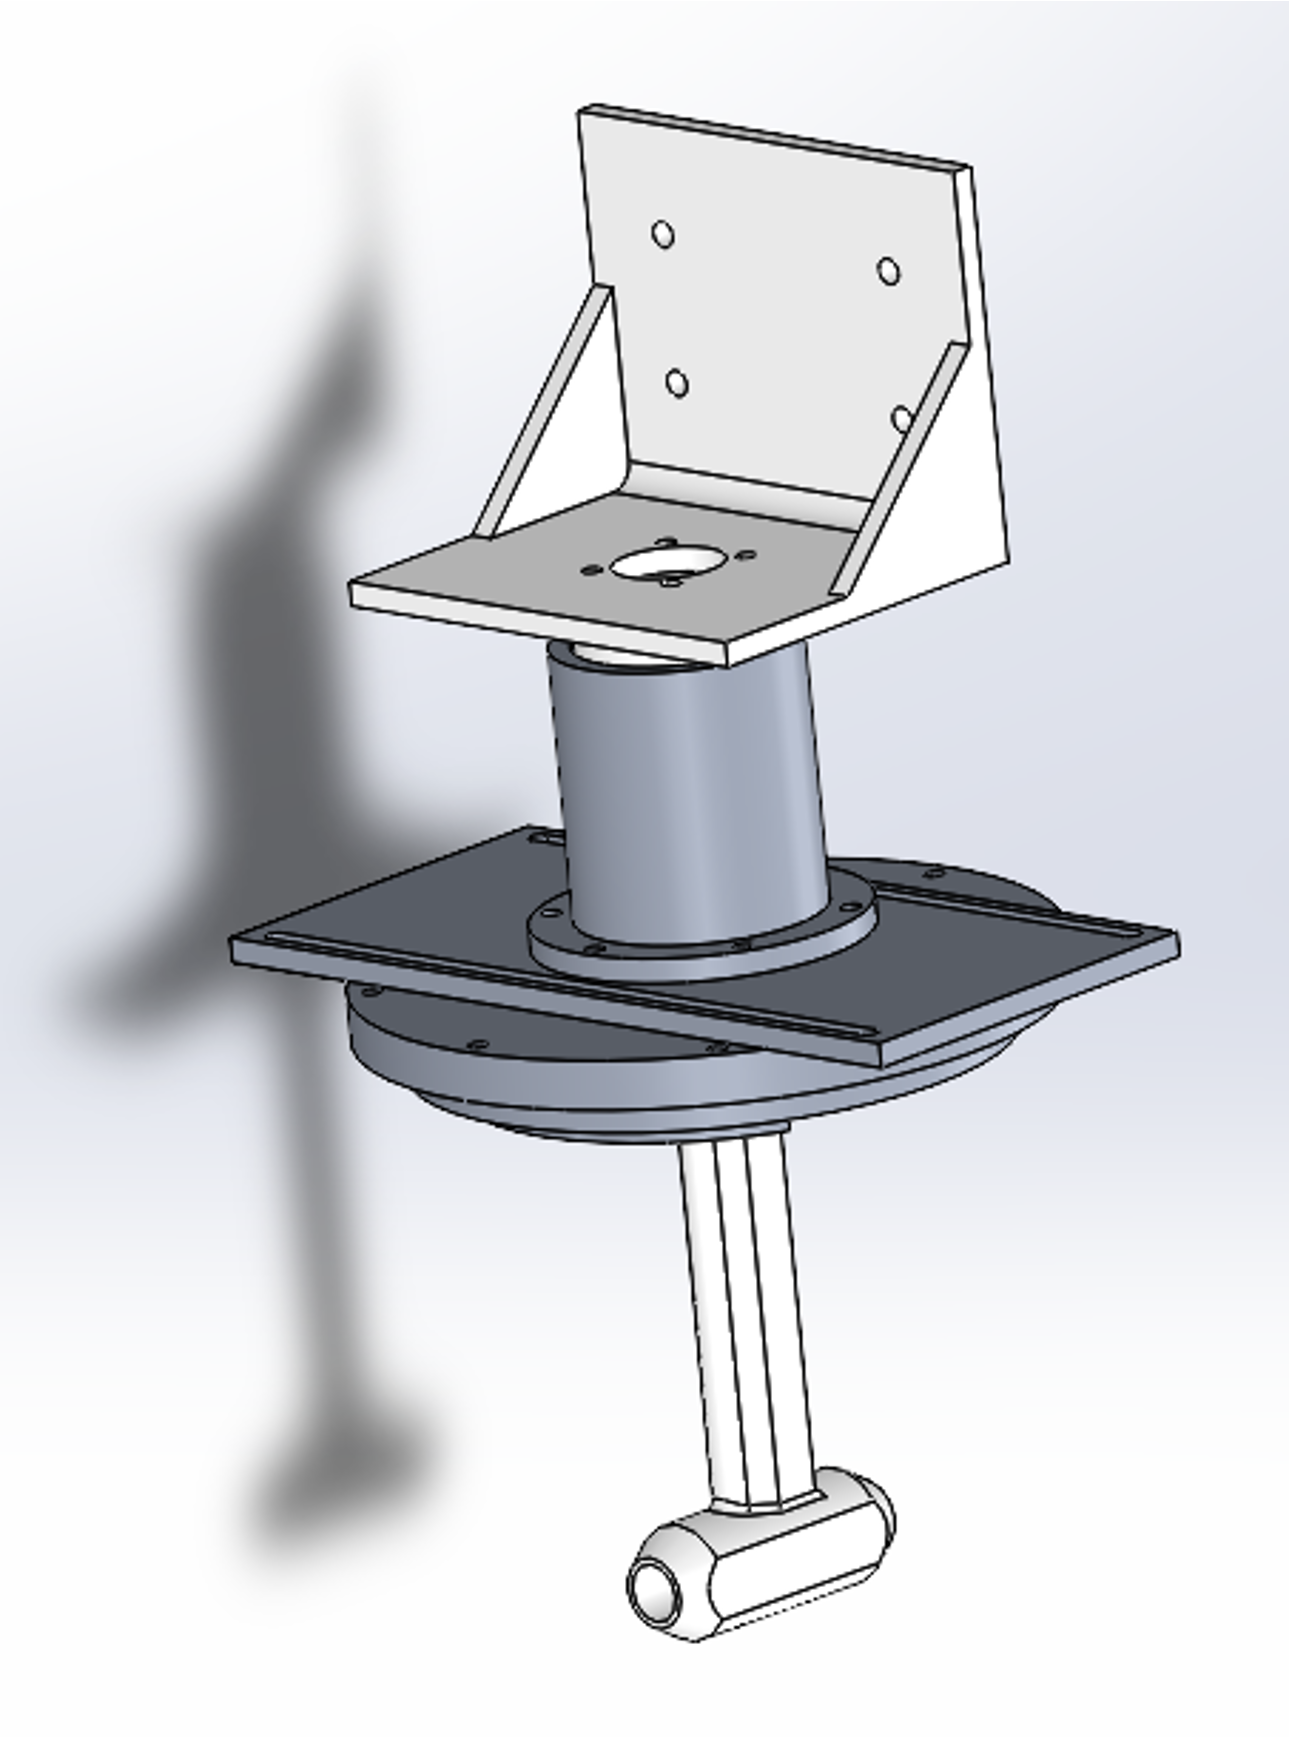
\includegraphics[width=\textwidth]{traverse-x}
        \caption{X traverse}
        \label{fig:traverse-x}
    \end{subfigure}
    \begin{subfigure}[b]{0.22\textwidth}
            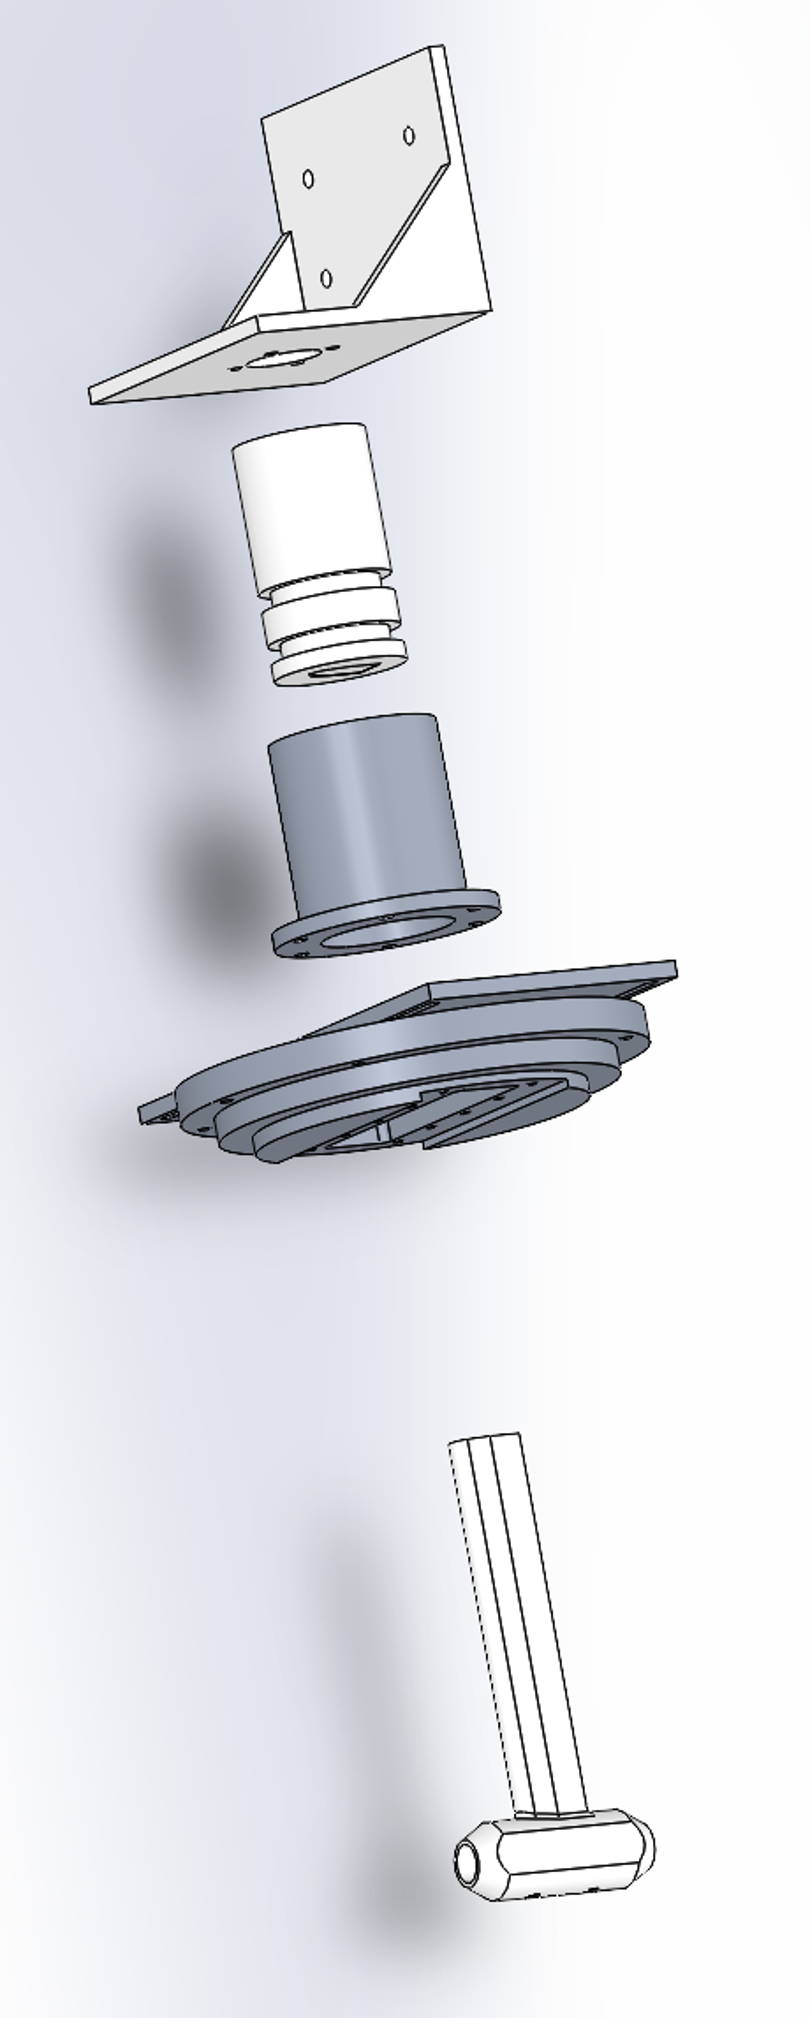
\includegraphics[width=\textwidth]{traverse-explode}
        \caption{Exploded assembly}
        \label{fig:traverse-explode}
    \end{subfigure}
    \begin{subfigure}[b]{0.35\textwidth}
            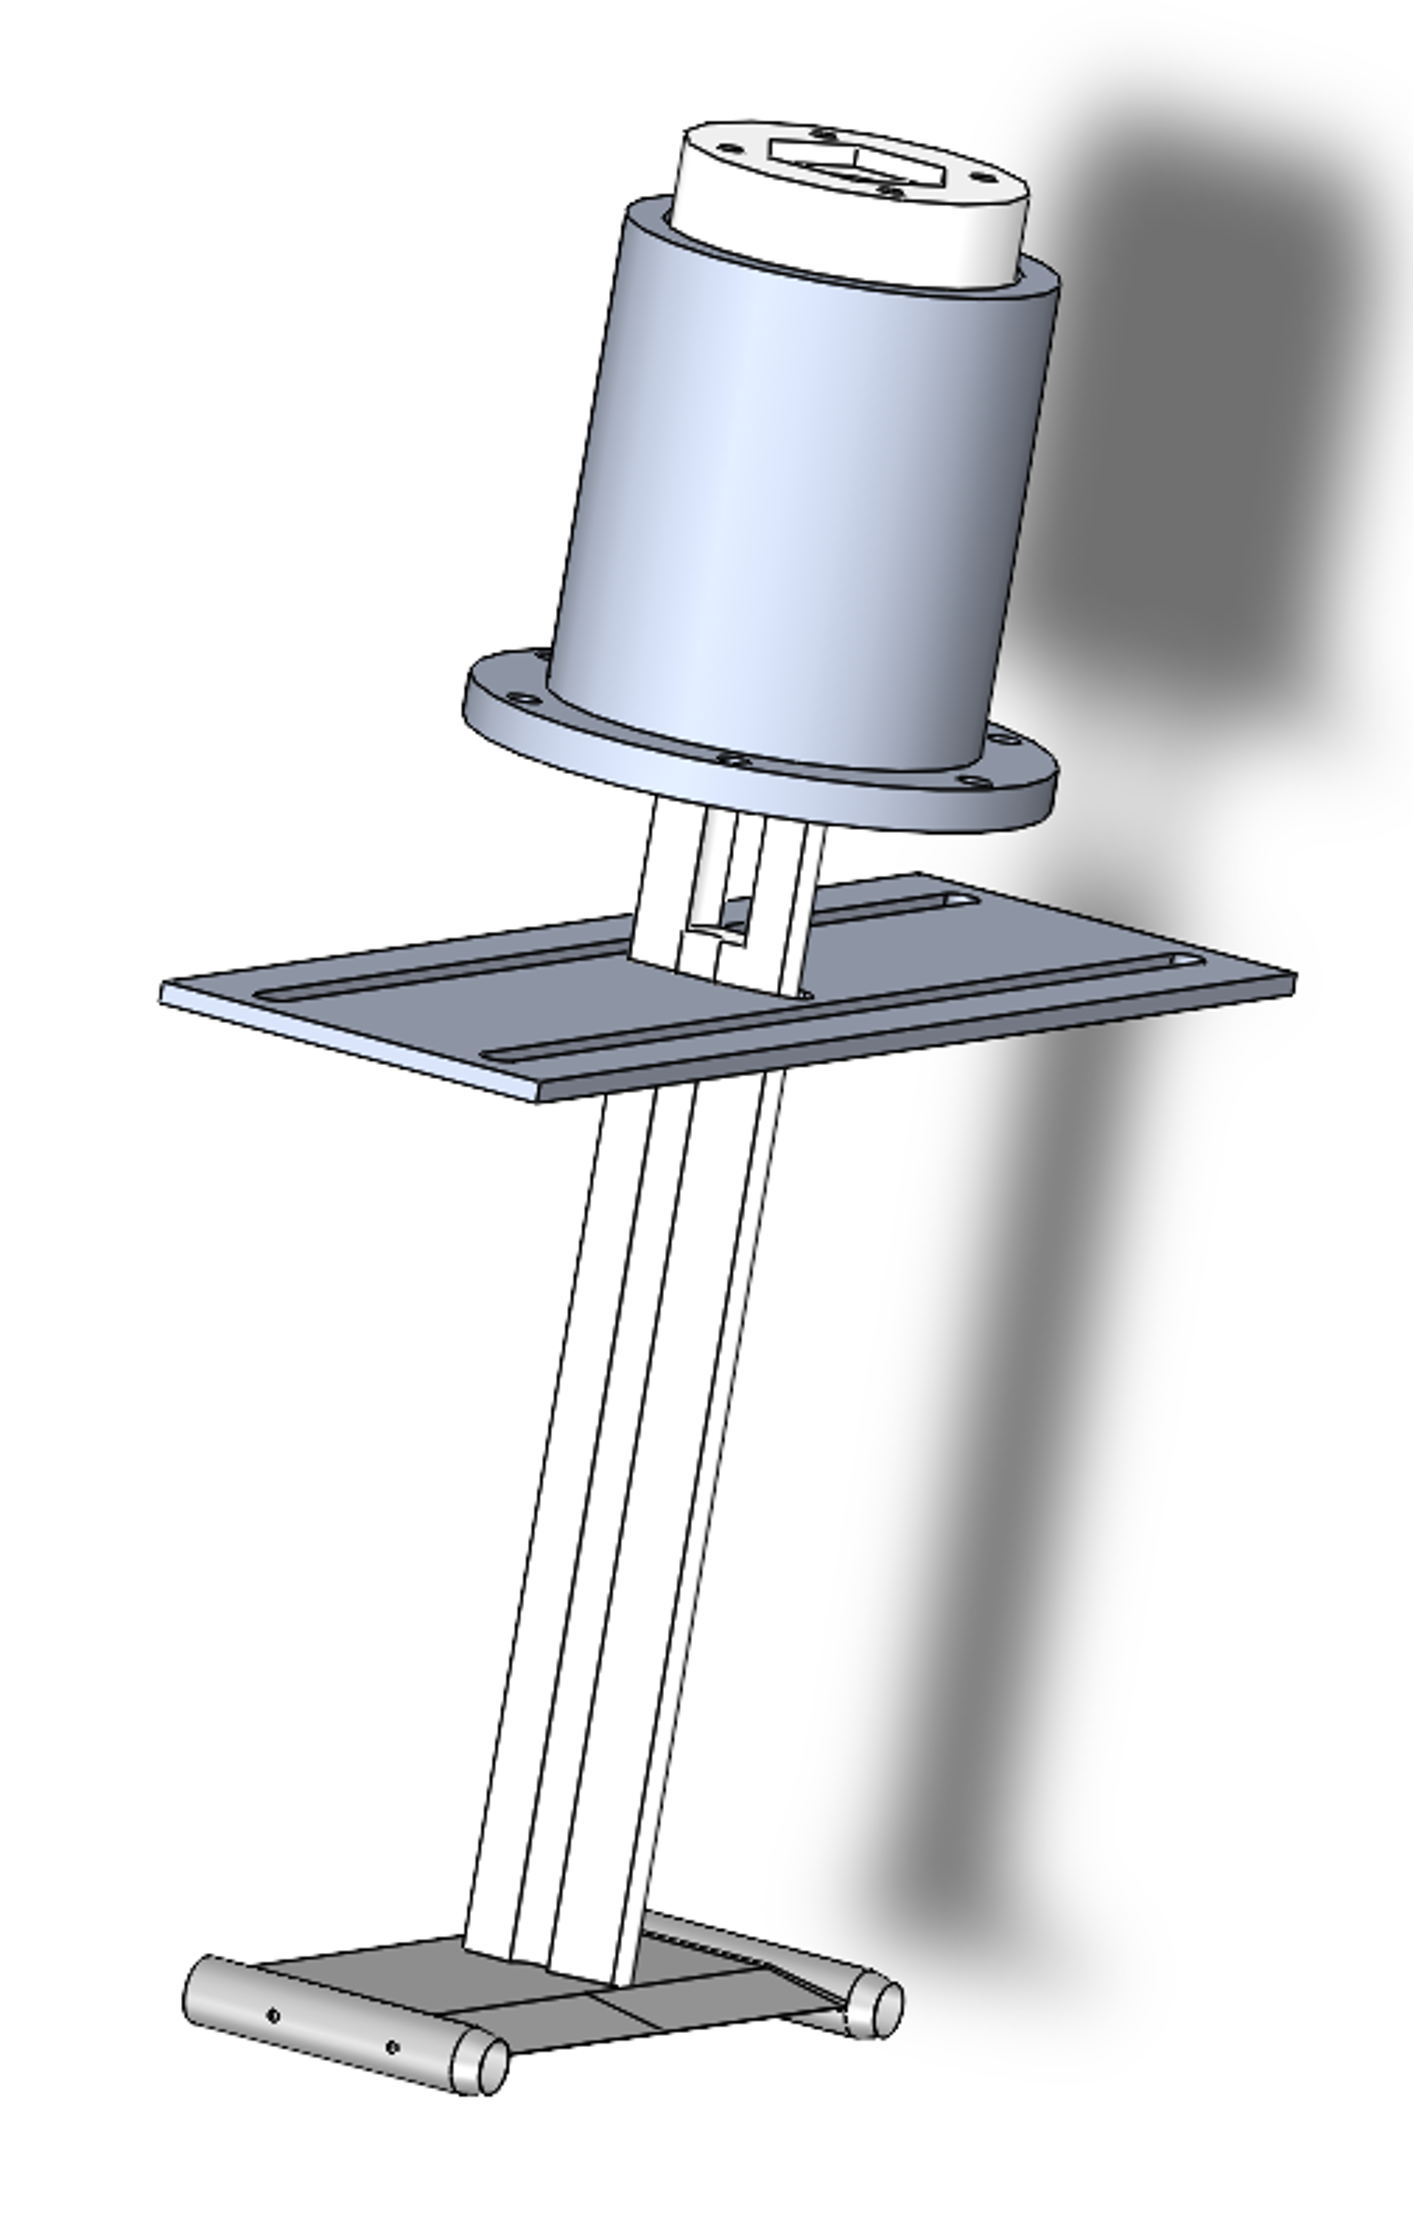
\includegraphics[width=\textwidth]{traverse-y}
        \caption{Y-traverse}
        \label{fig:traverse-y}
    \end{subfigure}
    \caption{Traverse configurations}
    \label{fig:traverse}
\end{figure}

\begin{figure}[ht]
    \centering
    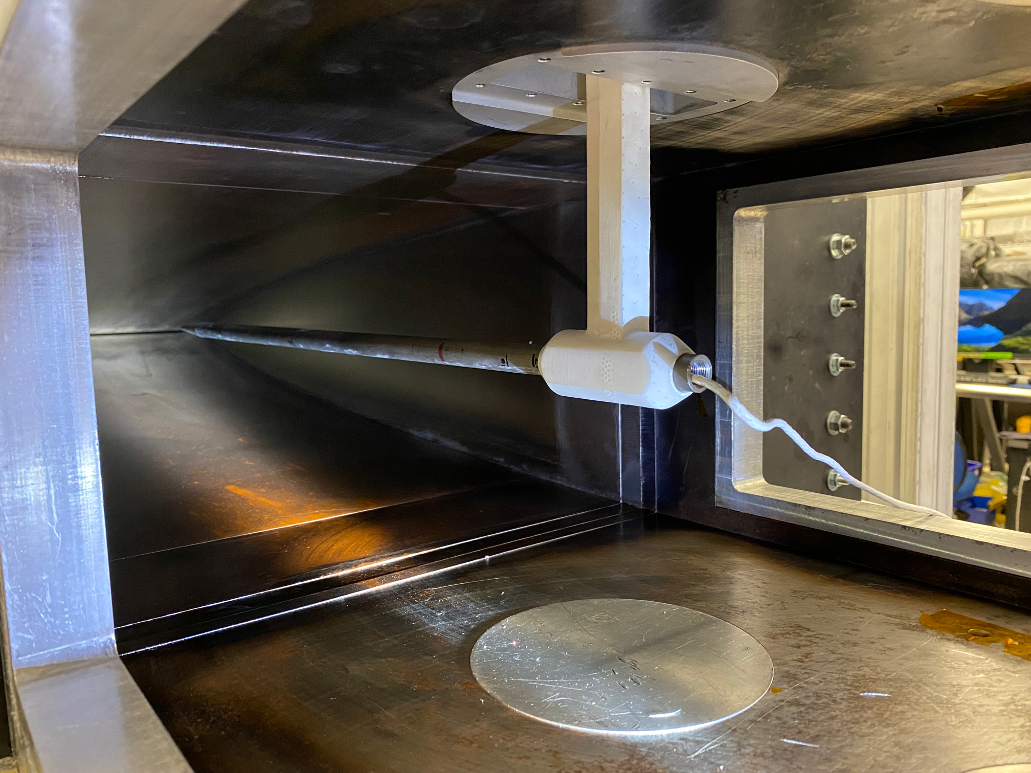
\includegraphics[width=6in]{pitot17}
    \caption{Pitot probe measuring 17 in. upstream of nozzle exit.}
    \label{fig:pitot17}
\end{figure}

\begin{table}[ht]
    \centering
    \label{tab:ace-survey}
    \begin{tabular}{|c|c|c|c|c|}
        \hline
    \textbf{Run} & \textbf{X (in.)} & \textbf{Y (in.)} & \textbf{Z (in.)} & \textbf{Re/m ($\times10^6$)} \\ \hline
        1 & 0 & 0 & 0 & 2$\to$7$\to$2 \\ \hline
        2 & -17 & 0 & 0 & 2$\to$7$\to$2 \\ \hline
        3 & -24 & 0 & 0 & 2$\to$7$\to$2 \\ \hline
    \end{tabular}
    \caption{Test matrix for preliminary noise hysteresis in ACE.}
\end{table}

\begin{table}[ht]
    \centering
    \label{tab:ace2-survey}
    \begin{tabular}{|c|c|c|c|c|c|}
        \hline
        \textbf{Run} & \textbf{X (in.)} & \textbf{Y (in.)} & \textbf{Z (in.)} & \textbf{Mach} & \textbf{Re/m ($\times10^6$)} \\ \hline
        1 & 0 & 0 & 0 & 6 & 2$\to$7$\to$2 \\ \hline
        2 & 0 & 0 & 0 & 5$\to$8$\to$5 & 3 \\ \hline
        3 & 0 & -3 & -3:1:3 & 6 & 3 \\ \hline
        4 & 0 & -1.5 & -3:1:3 & 6 & 3 \\ \hline
        5 & 0 & 0 & -3:1:3 & 6 & 3 \\ \hline
        6 & 0 & 1.5 & -3:1:3 & 6 & 3 \\ \hline
        7 & 0 & 3 & -3:1:3 & 6 & 3 \\ \hline
        8 & -6 & 0 & 0 & 6 & 2$\to$7$\to$2 \\ \hline
        9 & -6 & 0 & 0 & 5$\to$8$\to$5 & 3 \\ \hline
        10 & -6 & -3 & -3:1:3 & 6 & 3 \\ \hline
        11 & -6 & -1.5 & -3:1:3 & 6 & 3 \\ \hline
        12 & -6 & 0 & -3:1:3 & 6 & 3 \\ \hline
        13 & -6 & 1.5 & -3:1:3 & 6 & 3 \\ \hline
        14 & -6 & 3 & -3:1:3 & 6 & 3 \\ \hline
        15 & -17 & 0 & 0 & 6 & 2$\to$7$\to$2 \\ \hline
        16 & -17 & 0 & 0 & 5$\to$8$\to$5 & 3 \\ \hline
        17 & -24 & 0 & 0 & 6 & 2$\to$7$\to$2 \\ \hline
        18 & -24 & 0 & 0 & 5$\to$8$\to$5 & 3 \\ \hline
        19 (1) & 0 & 0 & 0 & 6 & 2$\to$7$\to$2 \\ \hline
        20 (2)& 0 & 0 & 0 & 5$\to$8$\to$5 & 3 \\ \hline
        21 (3) & 0 & -3 & -3:1:3 & 6 & 3 \\ \hline
        22 (4) & 0 & -1.5 & -3:1:3 & 6 & 3 \\ \hline
        23 (5) & 0 & 0 & -3:1:3 & 6 & 3 \\ \hline
        24 (6) & 0 & 1.5 & -3:1:3 & 6 & 3 \\ \hline
        25 (7) & 0 & 3 & -3:1:3 & 6 & 3 \\ \hline
    \end{tabular}
    \caption{Test matrix for ACE2.0 characterization and hysteresis study.}
\end{table}

\subsection{Uncerntainty Quantification}

Reference \cite{stephens-hubbard} and \cite{curriston} for how to proceed. Both repeat and replicate data...

\subsection{Hysteresis}

Dynamic sweeps of both Mach number and Reynolds number will be explored to determine any hysteresis effects in either the noise or the control parameters. Specifically, this will be accomplished in runs 1,2,8,9, and 15-20 in Table \ref{tab:ace2-survey}.

\section{Model Flow Characteristics Hysteresis During Mach Trajectory and Oscillation}

This objective will primarily serve as a demonstration of the capabilities for ACE2.0, but it will also provide preliminary insight into the hysteretic behaviour of dynamic Mach number experiments. The various flow characteristics that will be explored include shock interactions, boundary layers, and subsequent surface heat flux using schleiren and IR thermography.

The experiments here will follow closely with the work of Wirth \cite{wirth} to compare measurents from the dynamic runs to his results with the fin-cone model. This model, shown in Figure \ref{fig:fin-cone}, consists of a 7$\degree$ half-angle cone body with a single fin at an angle of 8$\degree$ from the body surface. The specific model used by Wirth will be used for these experiments as well. This physical, shown in Figure , was 3D printed with a ceramic-like material using SLA... The entire model is 15 inches long with the fin beginning 4 inches from the nose tip. The nose tip for this model has a radius of 0.0025 inches. 

Use fin-cone model for public and HARV for army and verbal?

\begin{figure}[ht]
    \centering
    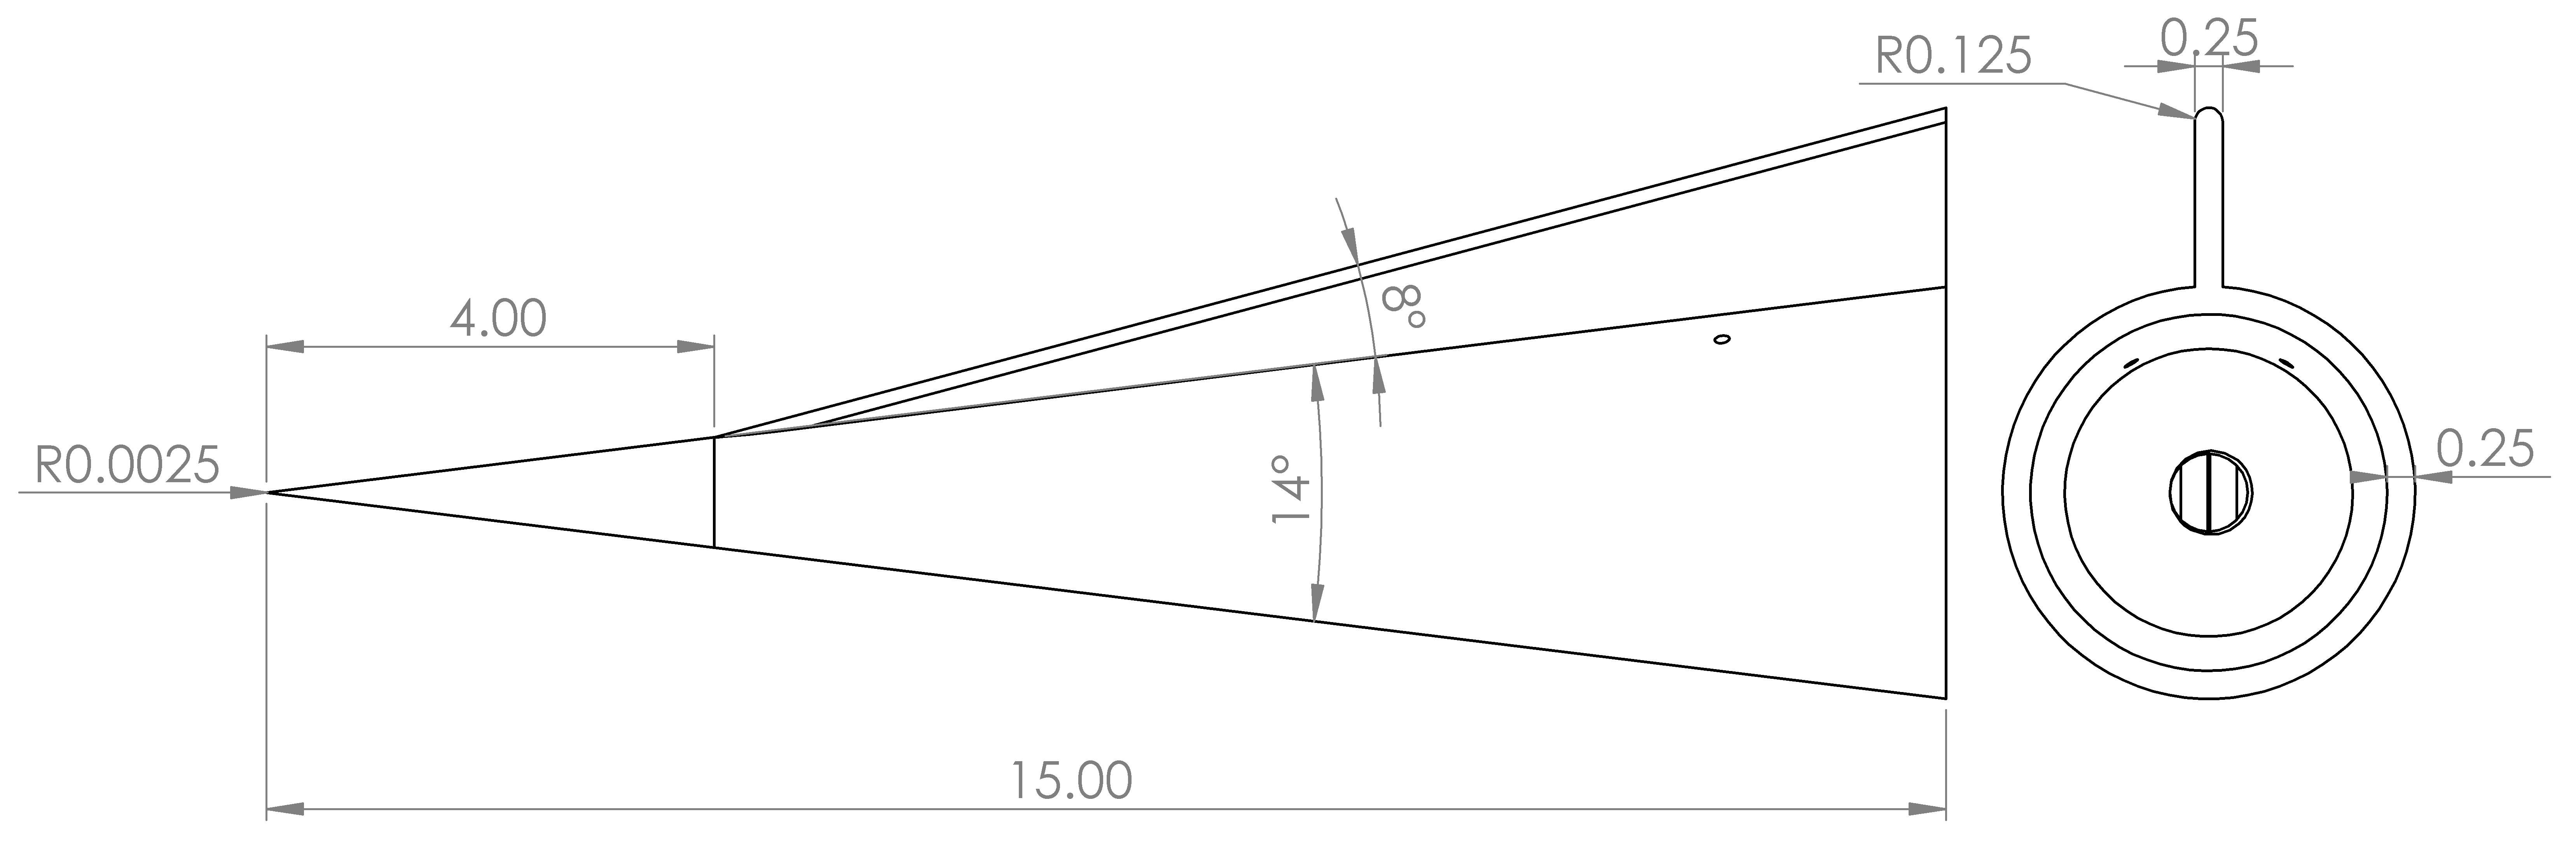
\includegraphics[width=6.5in]{fin-cone}
    \caption{Drawing of 7$\degree$ half-angle fin-cone model used for heat flux hysteresis study.}
    \label{fig:fin-cone}
\end{figure}

